\chapter{Diseño de algoritmo}
\section{Introducción}
En este capítulo se pretende abordar el diseño para llevar a cabo el objetivo principal y algunos de los específicos del proyecto.

\section{Diseño general de trabajo}
En la figura \ref{fig:esquema} se observan las partes que componen el trabajo del sistema. En este sentido, es necesario hacer una diferenciación entre la parte \textit{offline} y la parte \textit{online} ya que cada parte por separado conlleva requerimientos específicos.

\begin{figure}[h!]
    \centering
    \begin{subfigure}[b]{0.7\textwidth}
        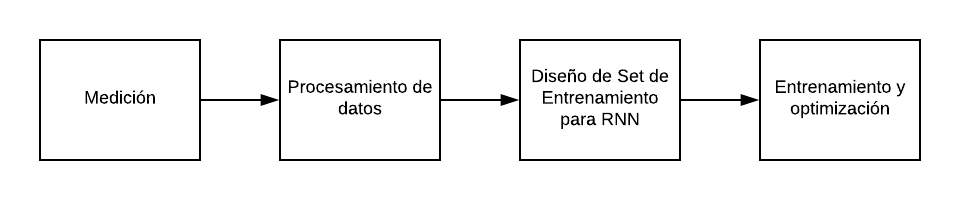
\includegraphics[width=\textwidth]{./images/online}
        \caption{Etapa Online}
        \label{fig:Online}
    \end{subfigure}
    
    \begin{subfigure}[b]{0.4\textwidth}
        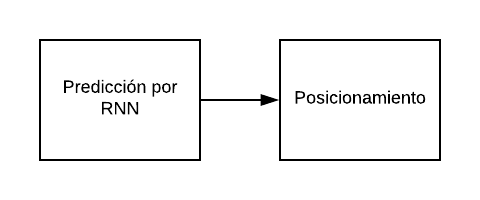
\includegraphics[width=\textwidth]{./images/offline}
        \caption{Etapa Offline}
        \label{fig:offline}
    \end{subfigure}
    \caption{Diagrama General de operación de Algoritmo de posicionamiento}
    \label{fig:esquema}
\end{figure}

\subsection{Offline}
\subsubsection{Medición}

En éste módulo se extraerán los datos usando como hardware, un ordenador de placa reducida como es Raspberry Pi 2 y un Adaptador USB Nano Inalámbrico N de 150Mbps, modelo TL-WN725N. Los cuales tendrán por función medir los niveles de intensidad de potencia de cada uno de los Access Points que se hallen a su alrededor.

% A través del comando \texttt{iwlist}, parte del paquete de herramientas de \texttt{wireless-tools} se recolectarán los niveles de intensidad de señal, las MAC de los AP, así como también del \ac{ESSID} de las redes.

% Para la medición, se dividirá el laboratorio tal que quede como una matriz de 3x3, 3 sectores a lo ancho y 3 a lo largo.

\subsubsection{Extracción y procesamiento de datos}

Para este módulo se trabajará con un algoritmo diseñado cuya función es hacer el pre-procesamiento de los datos. Esto se traduce en que el algoritmo escribe todos la información recopilada en un archivo que posteriormente es leído para filtrar de este sólo los datos que requerimos, esto es; la MAC del AP, el \ac{ESSID}, así como el \ac{RSSI}. Luego, el archivo obtenido corresponde al dataset de entrenamiento que será el usado entrenar la red.

\subsubsection{Diseño de Set de Entrenamiento}

Con el objetivo de relacionar los Niveles de Intensidad de Señal Recibida, con una posición en particular, es menester asociar estos a coordenadas en el espacio, para ello en este punto se leerá el archivo obtenido en puntos anteriores y coordenadas presentadas como pares ordenados, serán incorporados como un elemento más al dataset de entrenamiento.

\subsubsection{Entrenamiento y Optimización}

Dado que en principio, la red es incapaz de percibir la relación existente entre la posición y la densidad de potencia radiada, es preciso relacionar los datos con que se alimenta la red. Por esta razón es necesario hacer un ajuste adicional sobre estos.

Para que el sistema aprenda, es preciso que el dataset sea tan robusto como se pueda. Sin embargo, en lo que respecta a redes neuronales conceptos como  sobreajuste(\textit{\glsenablehyper\gls{Overfitting}}) y  subajuste(\textit{\glsenablehyper\gls{Underfitting}}) llevan a poner especial cuidado en que el sistema, con un número óptimo de iteraciones, datos y neuronas, funciones de activación y capas, alcance efectivamente el resultado deseado.

Por ello se implementarán técnicas de optimización de redes neuronales que cuidarán que los parámetros antes mencionados no lleven a resultados que sean distintos de los óptimos.

\subsection{Online}

\subsubsection{ANN para estimar la posición del objetivo.}

En este punto, se tomarán nuevas muestras de intensidad de señal a fin de entregarlas valores de prueba para predecir, según lo que aprendió la red en su entrenamiento, cuaĺ es la posición en que se haya el objetivo.

Como salida de la red se tendrá la posición y la precisión con que esta fue estimada.